
\section{Method Description}

\subsection{The Dataset Collection}
\begin{frame}
  \frametitle{Dataset Collection}
  \begin{figure}[!t]
    \centering
    \begin{minipage}[h]{0.32\linewidth}
        \begin{block}{exiD}
            \centering
            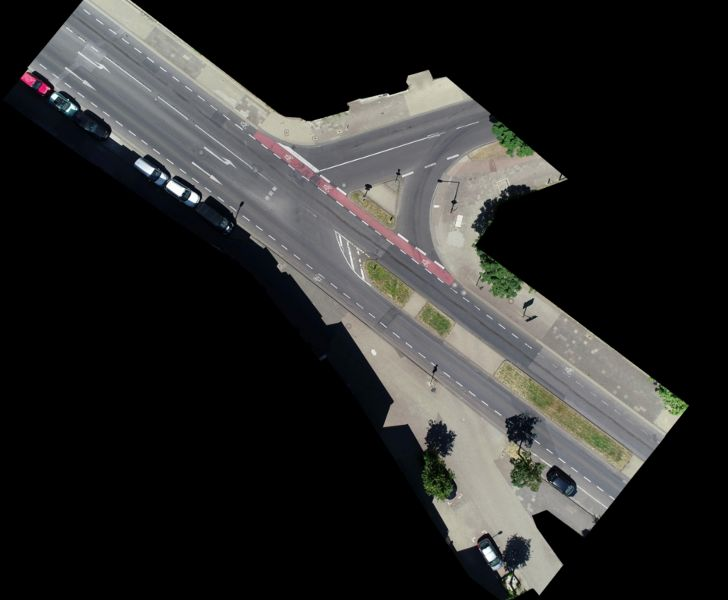
\includegraphics[width=\textwidth]{figures/pictures_first_part/inD.jpeg}
        \end{block}
    \end{minipage}
    \begin{minipage}[h]{0.32\linewidth}
        \begin{block}{rounD}
            \centering
            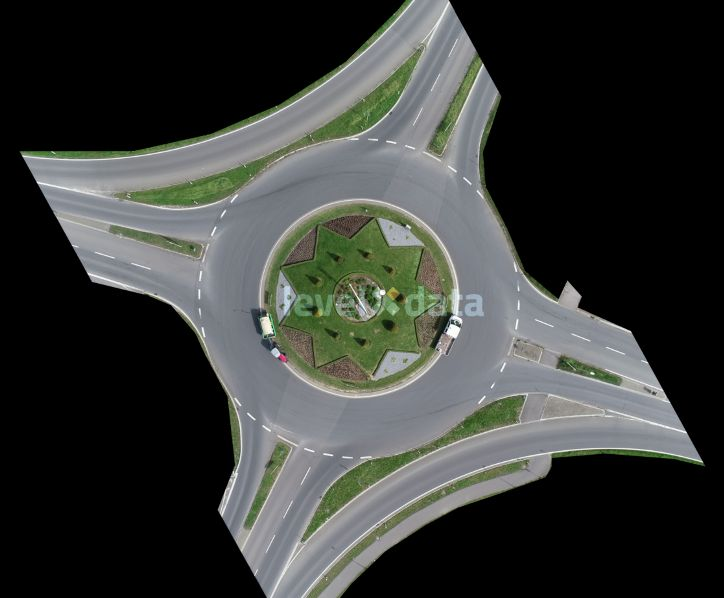
\includegraphics[width=\textwidth]{figures/pictures_first_part/rounD.jpeg}
        \end{block}
    \end{minipage}
    \begin{minipage}[h]{0.32\linewidth}
        \begin{block}{inD}
            \centering
            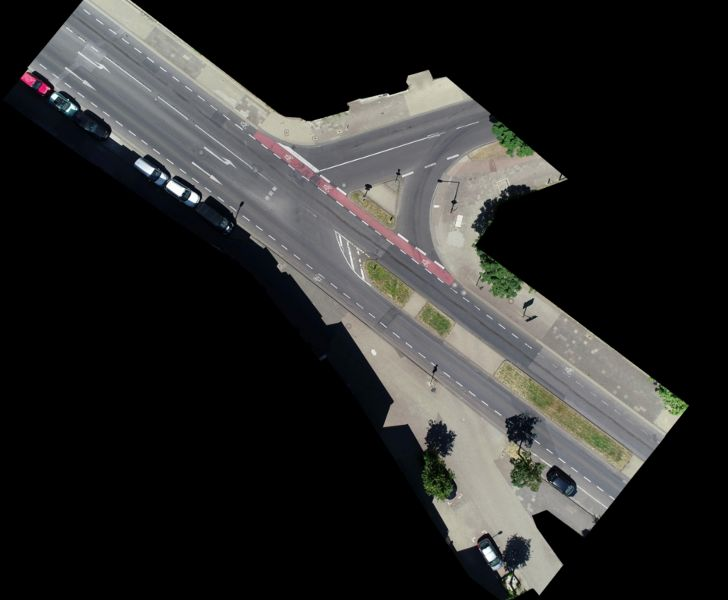
\includegraphics[width=\textwidth]{figures/pictures_first_part/inD.jpeg}
        \end{block}
    \end{minipage}
  \end{figure}
\end{frame}

\begin{frame}
  \frametitle{Method Description - Overview}
    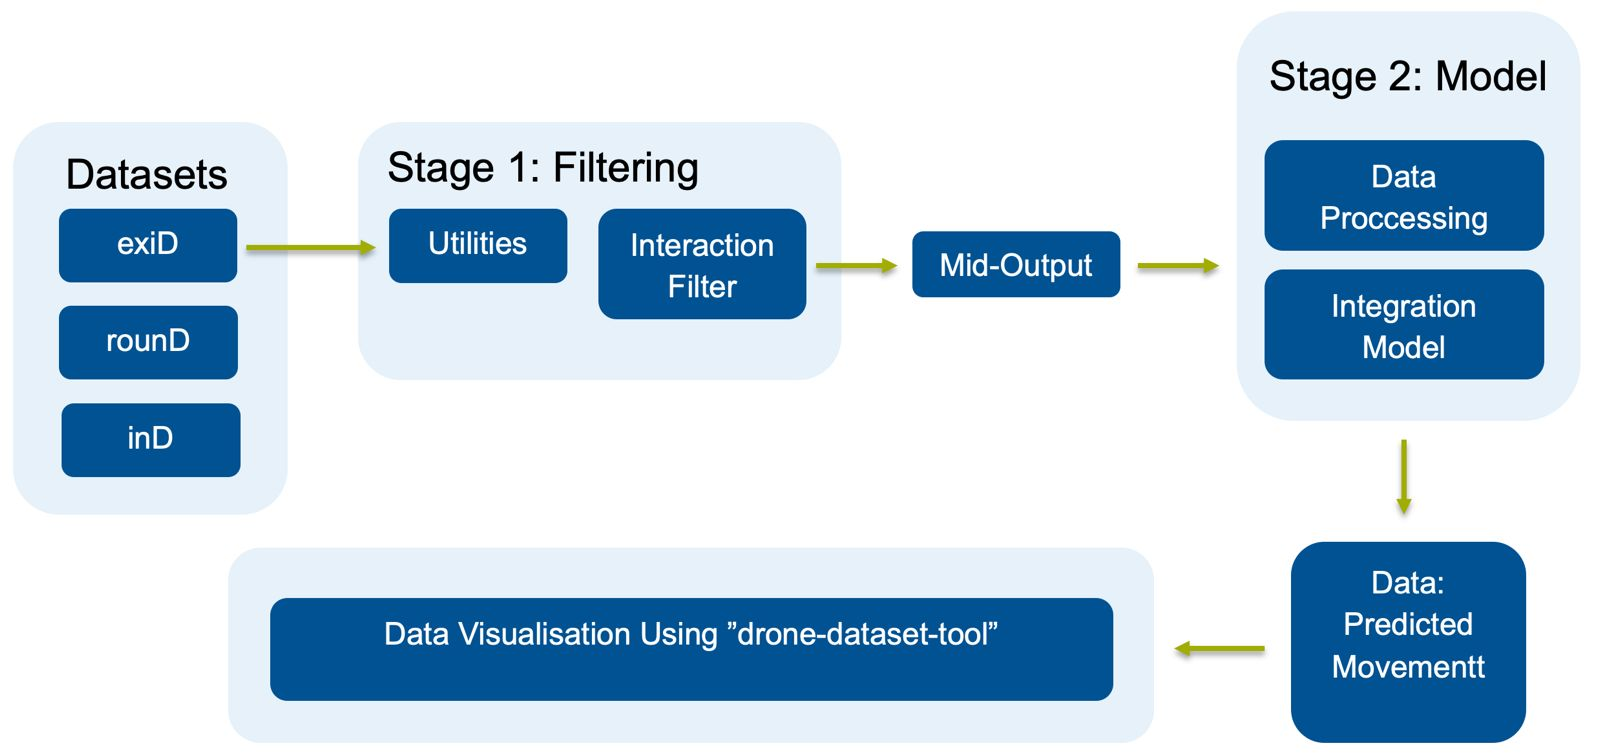
\includegraphics[width=\textwidth]{figures/pictures_first_part/method_overview.jpeg}
\end{frame}

\subsection{Stage 1 - Filtering process}

\begin{frame}
  \frametitle{Method Descripion - Stage 1}
    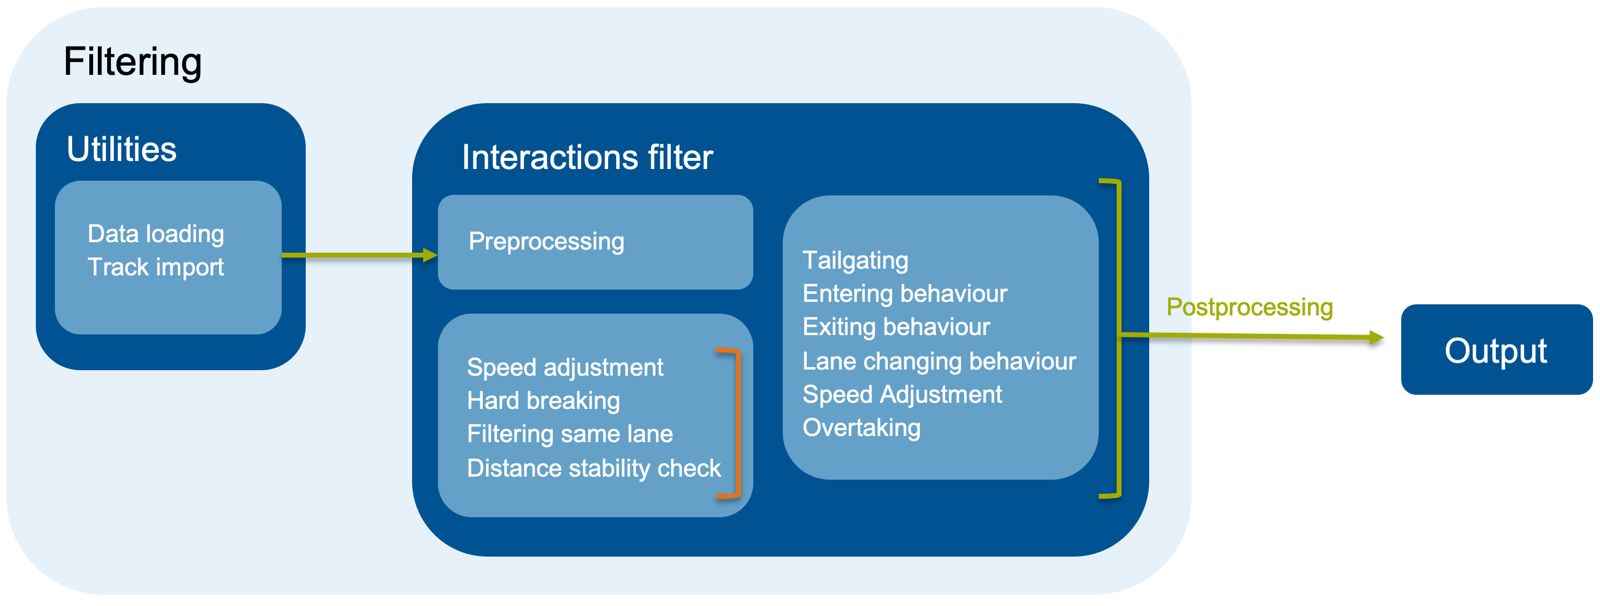
\includegraphics[width=\textwidth]{figures/pictures_first_part/filtering_overview.jpeg}
\end{frame}


\begin{frame}

  \frametitle{Method Descripion - Stage 1}
  \begin{figure}

    \centering
    \begin{minipage}[b]{0.49\linewidth}
        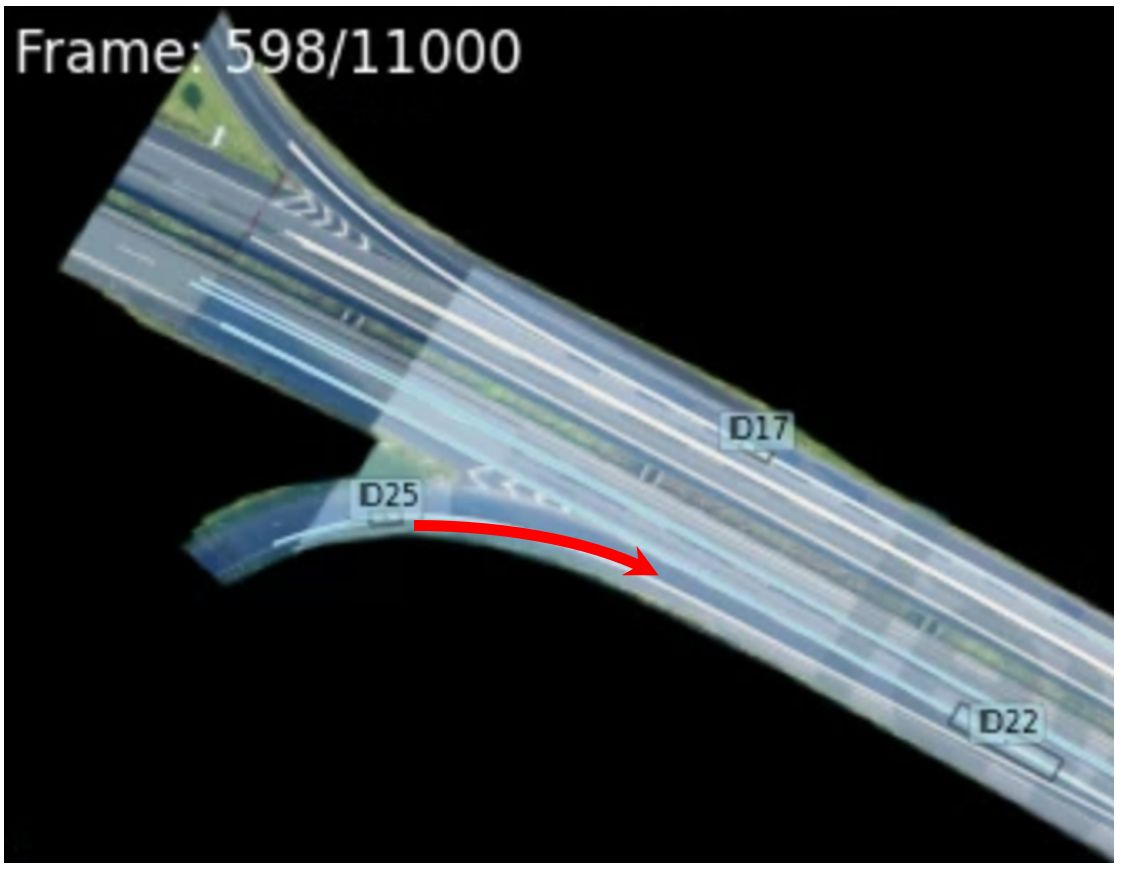
\includegraphics[width=\textwidth]{figures/pictures_first_part/street_with_arrow.jpeg}

        \centering \footnotesize Merging Lane Entering Scenario
    \end{minipage}
    \begin{minipage}[b]{0.49\linewidth}

        \centering
        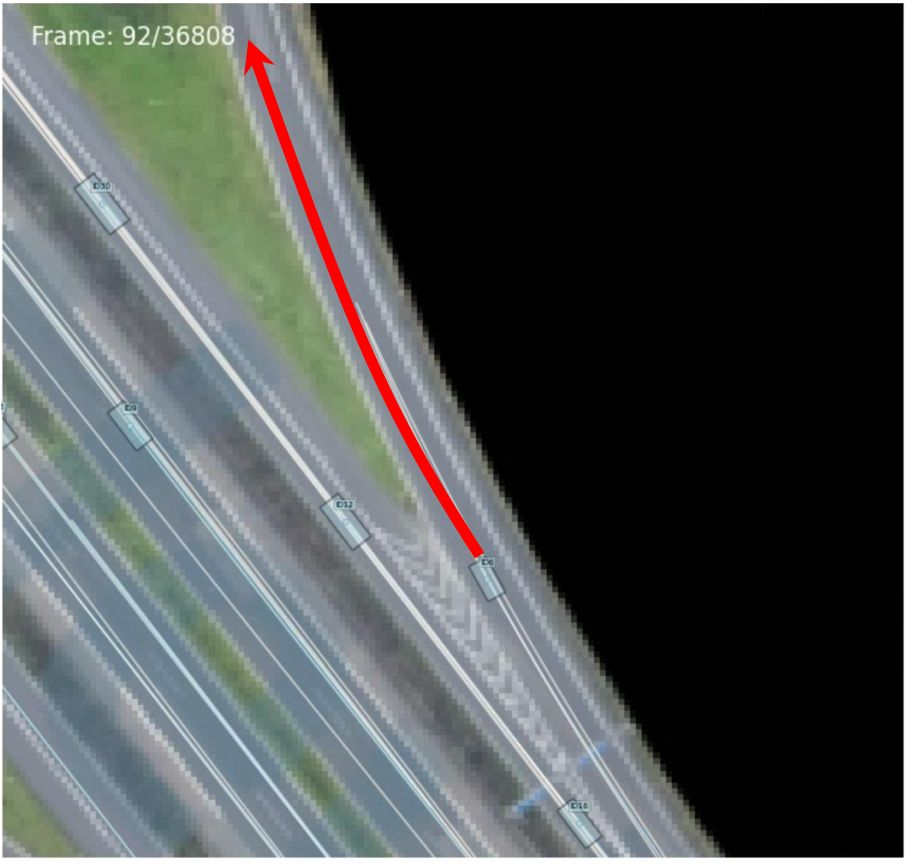
\includegraphics[width=0.82\textwidth]{figures/pictures_first_part/street_with_arrow_2.jpeg}

        \centering \footnotesize Merging Lane Exiting Scenario
    \end{minipage}
  \end{figure}
\end{frame}







\begin{frame}
  \frametitle{Method Descripion - Stage 1}

  \begin{figure}

    \begin{minipage}[b]{0.64\linewidth}
      \textbf{Filtering Stage: Identifying Vehicle \\ Behaviors}
      \begin{itemize}
          \item Preprocessing
          \item Behavior Detection
              \begin{itemize}
                  \item Entering/Exiting Behavior
              \end{itemize}
          \item Interaction Analysis
          \item Lane Change Detection
          \item Thresholds and Conditions
          \item Data Grouping and Sorting
      \end{itemize}
    \end{minipage}
    \begin{minipage}[b]{0.35\linewidth}

        \centering
        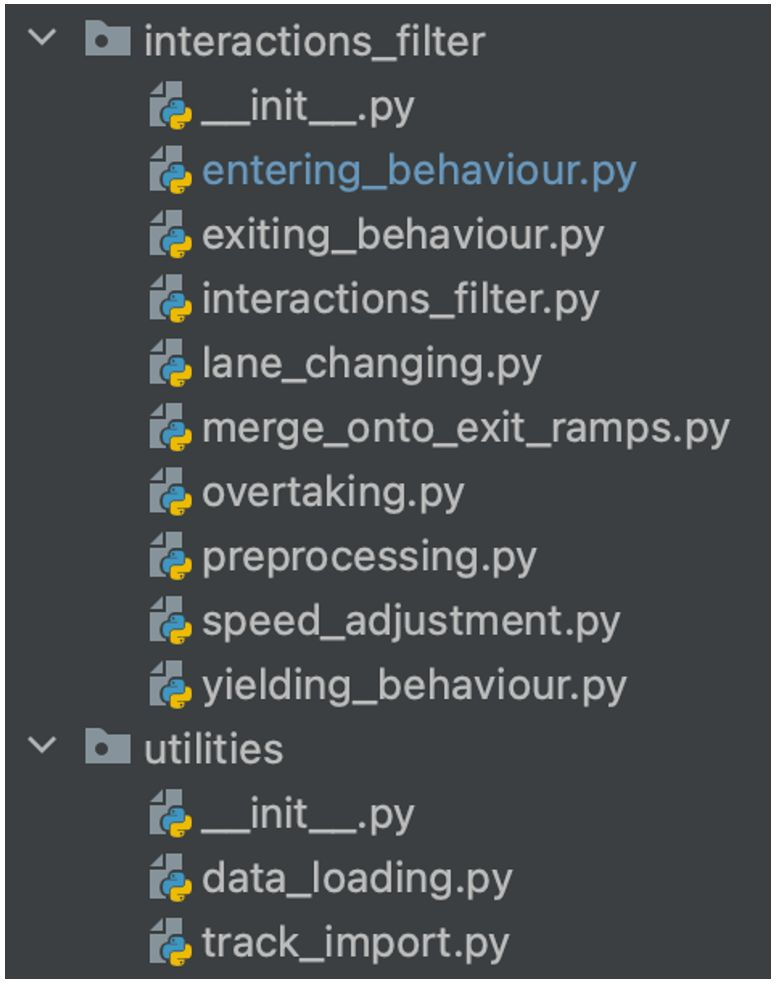
\includegraphics[width=1\textwidth]{figures/pictures_first_part/python_code_filter.jpeg}
    \end{minipage}
  \end{figure}
\end{frame}

\subsection{Stage 2 - Integration Model}

\begin{frame}
  \frametitle{Previous Integration Model }
    Distance and Velocity Equations (Ballistic Integration):
    \onslide<2, 3, 4>{
    \begin{align*}
        s(k+1) &= s(k) + dt \cdot v(k) + \frac{dt^2}{2} \color{blue}{a(k)} \\
        v(k+1) &= v(k) + dt \cdot                       \color{blue}{a(k)}
    \end{align*}

    }
    \onslide<3, 4>{

    \hfil

    Acceleration Equations (Rearranged):
    \begin{align*}
    \color{blue}{a(k)} &= \frac{2}{dt^2} \Bigl( s(k+1) - s(k) - dt \cdot v(k) \Bigr)\\
    \color{blue}{a(k)} &= \frac{1}{dt} \Bigl( v(k+1) - v(k) \Bigr)
    \end{align*}
    }
    \onslide<4>{

      \textbf{Problem:} Accelerations are not equal!
    }
\end{frame}


\begin{frame}
  \frametitle{Our Integration Model}
    Distance and Velocity Equations:
\onslide<2, 3, 4>{
    \begin{align*}
    s(k+1) &= s(k) + dt \cdot v(k)+ \textcolor{red}{c_1} a(k) + \textcolor{red}{c_2} a(k-1) \\
    v(k+1) &= v(k) +                \textcolor{red}{c_3} a(k) +                \textcolor{red}{c_4} a(k-1)
    \end{align*}

    \hfil
}
\onslide<3, 4>{

    Acceleration Equations:
    \begin{align*}
    a(k) &= - \overline{\textcolor{red}{c_1}} a(k-1)  + \overline{\textcolor{red}{c_2}} \bigl( s(k+1) - s(k) - dt \cdot  v(k)\bigr)\\
    a(k) &= - \overline{\textcolor{red}{c_3}} a(k-1)  + \overline{\textcolor{red}{c_4}} \bigl( v(k+1) - v(k) \bigr) 
    \end{align*}

}
  \onslide<4->{
    $\Rightarrow$ This can be solved using linear regression.
  }


\end{frame}


